\begin{center}
    \section*{\fontsize{20}{20}\selectfont Chapter 1}
\end{center}
\vspace{10mm}
\section{Introduction}
Autism Spectrum Disorder (ASD) is a neurodevelopmental disorder that influences and also impacts the communication, social interactions, and behavior of a person in his childhood and later in life. ASD can normally occur in childhood and persist throughout life. Children with ASD tend to exhibit different behavior patterns, including problemetic with social communication, repetitive behavior and restricted or interests. Therefore early detection of autism is very crucial because it really enables a childran to get the right help and support for a normal life\cite{okoye2023early}.

Conventionally, the diagnosis of autism is carried out by observation, assessment, and the use of questionnaires by parents or professionals. However, this method is often time-consuming and sometimes expensive and prone to being ambiguity. But with the blessings of technology, machine learning and artificial intelligence have proven to be of great help in the early diagnosis of autism through the analysis of data related to behavior\cite{perochon2023digital}.

The primary goal of this research is to make an intelligent system that can identify children with Autism Spectrum Disorder using video footage data. In this study, machine learning techniques are used to analyze behavioral traits and identify specificpatterns associated with Autism Spectrum Disorder. The research focuses on computer vision-based techniques for identifying behavioral patterns, which can be used to enhance the accuracy of the prediction task.

This study tries to improve the early detecting of autism by designing a classifier that is strong and accurate. The classifier has a solution that is automated and can help medical professionals and researchers for classification tasks.



\subsection{Problem Statement}
Autism Spectrum Disorder (ASD) is a complex neurodevelopmental problem that effects the communication, social interaction, and behavior of children in a not so normal way. The early diagnosis of autism is highly significant as it can greatly help in improving the development and quality of life of children\cite{okoye2023early}. However, the current techniques being employed for the diagnosis of autism are primarily based on observation, behavior analysis, and questionnaires that are to be filled out by experts in the field or concerned parents. The traditional techniques are highly time-consuming, costly and may generate biased results based on the experience of the expert which is solely reliable on the respective persons expertise.

In most instances, the early diagnosis of the condition is often delayed due to a lack of medical resources, a lack of professionals and the complexity involved in the behavioral assessment process. In most cases, this can result in the child not getting the early intervention and support they need. In other words, the need for an efficient system that can identify autism early exists.

Recent advances in machine learning and AI open new opportunities for the analysis of behavioral data and the identification of patterns associated with ASD in a more efficient manner\cite{rajpurkar2022ai}. However, most of the current models still have issues with accuracy, generalization and the use of behavioral and visual data features.
\begin{figure}[htbp]
\centering
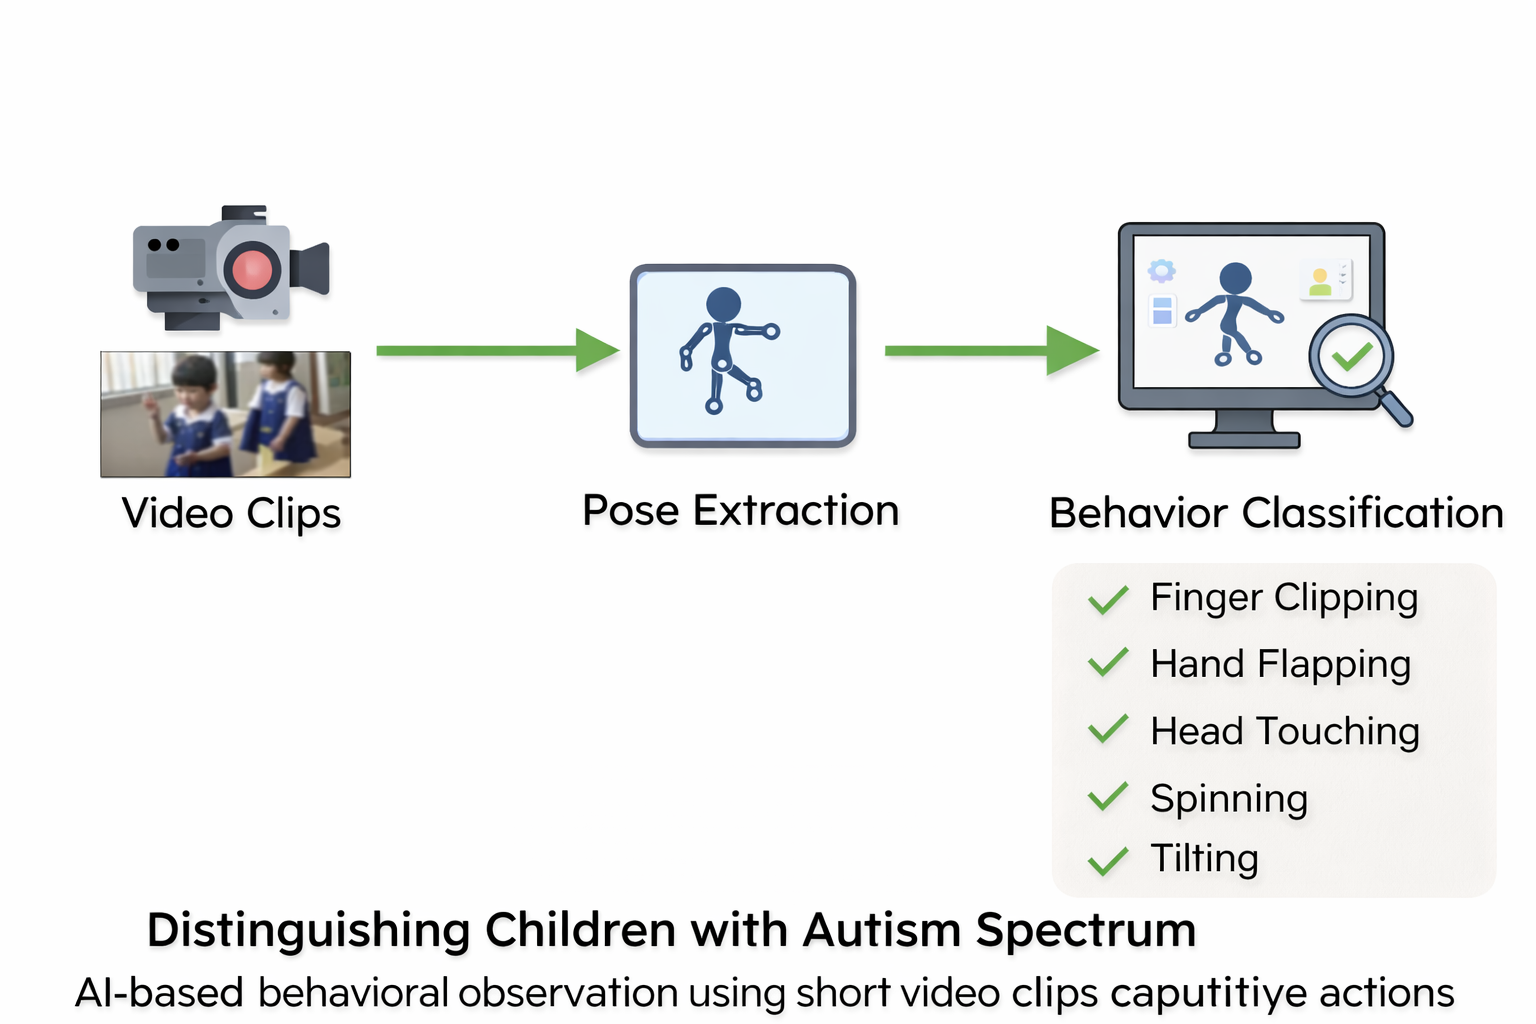
\includegraphics[scale=0.25]{image/intro.png}
\caption{Introductory Representation of the Thesis}
\label{fig:workflow}
\end{figure}

To overcome such problems, the proposed study intends to design a classification system based on machine learning to identify children with Autism Spectrum Disorder using behavioral information and computer vision. It will help in increasing the accuracy of predictions and designing a helpful tool for early autism screening to assist medical professionals and researchers.

\subsection{Problem Background}
Autism Spectrum Disorder (ASD) is a brain developmental disorder that impacts the communication, social interaction and behavior of affected toddlers especially later on life because in childhood it may seem cute but later on life it starts to get its awkward form.The term “spectrum” reflects the differences in the presence and severity of symptoms from child to child. While some children display minor symptoms, others face more difficulty in communicating and interacting socially. According to global health statistics, there has been a rise in the number of autism cases in the past few years.

Early detection of autism is a very crucial factor in enhancing the cognitive, social, and behavioral growth of a child\cite{okoye2023early}. If autism is detected in the early stage, fortunately, children can be provided with appropriate therapy, education, and support services that enable them to cope better with society and life. But the early detection of autism is a very difficult task because the symptoms of autism are quite diverse and may resemble other developmental disorders sometimes to intellect disorder.

At present, the diagnosis of autism is primarily dependent on behavioral observation, psychological assessment, and screening tests performed by medical professionals. The conventional diagnostic process is time-consuming and requires specialized knowledge and experience. In most developing nations, including those with less developed healthcare systems, access to specialized personnel and diagnostic facilities is not always available.Thus it might have led to a considerable delay in diagnosis and treatment for most children for sure.

With the improvement in technology, machine learning and artificial intelligence are becoming promising areas in the field of health care\cite{hossain2023smart}. Machine learning and artificial intelligence are capable of processing large data, showing hidden patterns and helping in the decision-making. In the study of autism, ML classifiers are implemented to process behavioral data and predict autism related traits. Recently, computer vision has been employed in the study and analysis of behavioral traits from visual data such as body language and social interactions.

However, despite these developments, current systems are still facing the challenge of giving high accuracy and feasibility in their implementation. Thus, the need for enhanced automated systems that can integrate behavioral analysis and computational methods for the early and accurate detection of autism traits is logical. This study is therefore informed by the need to address these obstacles by developing a data-driven system that can distinguish children with autism using machine learning and computer vision techniques.

\subsection{Research Objectives}
This research was progressed bearing some crucial objectives in the criteria. The objectives are very much feasible and not impossible to achieve. These objectives have been tried to acheive using open source tools and practical implementations. Below are those objects we tried to gain,
\begin{itemize}
    \item To examine and evaluate the behavioral traits related with Autism Spectrum Disorder in children.
    
    \item To create a machine learning model for the identification of children with Autism Spectrum Disorder and thus identifying children with austistic like features based on their behavioral traits and poses.
    
    \item To develop a systematic processing system for data preprocessing, feature extraction, model development, and evaluation.
    
    \item Investigating Computer vision application to get behavioral trait symptom from the visual and graphic data for autism detection.
    
    \item To assess the performance of the proposed system by using right methods and measures.
    
    \item Providing an assistive system that can help researchers or professionals of the area in the early screening of autism.
\end{itemize}


 
\subsection{Motivations}
Autism Spectrum Disorder (ASD) is increasingly observed in children across the globe sadly and it has a great effect on the social, behavioral, and communication skills of these innocent children. The early detection of autism is critical as it helps in improving the learning capacity of the might or might no be autistic child significantly. Well, in many instances, the diagnosis of autism takes place at a later platform due to the unavailability of specialists, the lengthy process of diagnosis, and the subjective assessment of the behavior of the child which is really a issue.

The lack of specialists and diagnostic is heavily seen in developing countries, thus it makes the early screening of autism even more difficult. This leads to the diagnosis of autism late, which further makes the early intervention programs ineffective thus making the children a burden to the society.

Again,recent advancements in machine learning and artificial intelligence have shown promising results in healthcare applications indeed, particularly in pattern recognition and data analysis fortunately. These technologies can analyze complex behavioral data and identify patterns that may not be easily noticeable through traditional methods with a great certain. Also, computer vision algorithms have new possibilities and opportunistic doors for analyzing behavioral clues from visual data, such as body movements and posture.

The motivation of this research arises from the need to combine data-driven machine learning methods with visual behavior analysis to support autism detection. By developing an automated and systematic pipeline, this study aims to decrease dependency on manual assessments and provide a supportive software(AI) tool that can create a path for the researchers and healthcare professionals to study for in this field. This work is also motivated by the potentiality to contribute to early screening systems that are more accurate, scalable and suitable for real-world applications out there.

\subsection{Significance of the Research}
This is important research because it aims to improve the early detection of Autism Spectrum Disorder (ASD) by machine learning and computer vision algorithms. Early detection of autism is critical for providing early intervention, which has a positive impact on the child’s social, behavioral, and cognitive development later on in its life.In addtion,with an automated solution, this research aims to help and improve current diagnosis methods too.

The system proposed has the potentiality to decrease dependency on time consuming and human dependent manual analysis of behavioral and visual information. Therefore, this can assist medical professionals and researchers in making more pre informed decisions and thus improving the efficiency of autism screening procedures. Machine learning algorithms enable the analysis of large amounts of data in a consistent way, potentially resulting in more accurate and reliable outcomes.
From the viewpoint of a technical standing, our study tries to make a contribution to the use of data-driven approaches in the area of autism research. The combination of a structured processing pipeline which consists of data preprocessing, feature extraction, model training, and evaluation offers a useful framework that can be expanded in future research. The investigation of computer vision based behavioral analysis also puts additional benefit by showing how visual features can be used with  traditional behavioral measures currently in use.

In summary, this study is important because it is trying to fill the gap between healthcare and technology in the developing coutries where it is very common. The results and approach of this study can be the pioneer for future research in the area of automated systems for screening autism and also provide a basis for further investigation into the use of artificial intelligence approaches for the analysis of neuro developmental disorders.
\subsection{Research Contribution}
We tried to contribute to this research thinking about it very much down to earth and our contribution has beed standarized with the implemention. Below are the exact contributions that we tried to contribut to this research,
\begin{itemize}
    \item This study proposes a holistic pose based video analysis system for autism related behavioral poses in children from raw video input to indentifying results.
    
    \item The MediaPipe Pose library is used for the extraction of human body landmarks from video footage data, thus giving the conversion of visual behavioral data into numerical data passed to machine learning for training.
    
    \item We were able to collect dataset of autism affected child about their repetitive traits like hand flapping, finger clipping, head touching, spining and tilting via the one to four seconds long footages which holds great potential for research purpose.

    \item We extracted sequences from this footages the train RNN base deep learning models to find interdepended frames of each traits to discover hidden relations among each traits.
    
    \item AI models were trained to recognised these behaviours of a autism child so that it can be later used for screening.
    
    \item Explainable AI analysis clearly shows the human body land marks pattern which leads the way to find key insights of these five traits
\end{itemize}



\subsection{Complex Engineering Analysis}

We tried to address the complex engineering problems first by exactly knowing what are the complex engineering problems applicable to this research. Below that attempt has been tried to fullfill.

\textbf{P1: Depth of Knowledge} \\
\textbf{K1 (Natural Science):} Undertanding the five repetitive patterns of human gestures that autism affected children make which are hand flapping, finger clipping, spining, head touching and tilting. \\
\textbf{K2 (Mathematics):} Usage of ROC-AUC curves, precision, recall, f1 score and macro average scores related to statistics  \\
\textbf{K3 (Engineering Fundamentals):} Preprocessing of the raw footages containing the five traits, feature extraction, sequence extraction, training models\\
\textbf{K4 (Specialist Knowledge):} MediaPipe Pose, machine learning, BiLSTM, CNN-BiLSTM, and explainable AI. \\
\textbf{K5 (Engineering Design):} Designing an automated pipeline from preprocess the raw footages to traing models with them and generating validated classification result.\\
\textbf{K6 (Engineering Practice):}On field practical data collected from the exact affected children \\
\textbf{K7 (Comprehension):} Realising ethical constraints, overfitting, paperworks, screening challanges. \\
\textbf{K8 (Research Literature):} Utilizing recent researches in the field and finding gaps.

\textbf{P2: Conflicting Technical Issues} \\
Balancing training and validating accuracy and other metrics with the limited dataset which has class imbalance and variable pose qualities.

\textbf{P3: Depth of Analysis} \\
Since it is a classification task, the study not only validates accuracy but also ROC-AUC curve,precision, recall, f1 scores, macro average scores and also the confusion matrice.

\textbf{P4: Familiarity of Issues} \\
The thesis tries to explore the less explored autism traits of children affected with it and combine the familiar deep learning and machine learning models for AI implication for assistive screening.

\textbf{P5: Extent of Application} \\
The propose thesis of ours can assist the researchers, special schools, clinics for primary screening of the suspected child.

\textbf{P6: Involvement of Stakeholders} \\
The application of this thesis involves children, parents, special school authorities, researchers and also the health care professionals.

\textbf{P7: Interdependence} \\
The thesis is a interdepended piple line of preprocessed data, AI models training and finally evaluating.

 
\subsection{Thesis/Project Organization}

This thesis is divided into a number of chapters each of which deals with a particular side of the research work.

Chapter 1: This is a indroductory chapter to the research work, which includes the background of the problem, problem statement, research objectives, motivation, significance of the research work, research contribution, and complex engineering analysis.

Chapter 2: This chapter deals with the literature review of Autism Spectrum Disorder, machine learning based autism detection, pose estimation, and video based behavior analysis.

Chapter 3: This chapter tries to explain the methodology of the proposed system by covering the entire processing pipeline, description of the dataset, video preprocessing, extracting of pose landmarks, data augmentation strategies, feature extraction, models and off course training.

Chapter 4: This chapter has the experimental results and performance analysis and it also covers comparison of models, validation results, confusion matrices, ROC-AUC curves, results of explainability analysis, and discussion of results.

Chapter 5: This chapter concludes the thesis by summarizing the research outcomes, limitations of the proposed approach, and the future work.


